% ---------
%  Compile with "pdflatex hw0".
% --------
%!TEX TS-program = pdflatex
%!TEX encoding = UTF-8 Unicode

\documentclass[11pt]{article}
\usepackage{jeffe,handout,graphicx}
\usepackage[utf8]{inputenc}		% Allow some non-ASCII Unicode in source
\usepackage{tikz}
\usetikzlibrary{automata, positioning}

%  Redefine suits
\usepackage{pifont}
\def\Spade{\text{\ding{171}}}
\def\Heart{\text{\textcolor{Red}{\ding{170}}}}
\def\Diamond{\text{\textcolor{Red}{\ding{169}}}}
\def\Club{\text{\ding{168}}}

\def\Cdot{\mathbin{\text{\normalfont \textbullet}}}
\def\Sym#1{\textbf{\texttt{\color{BrickRed}#1}}}

\newtheorem{Lemma}{lemma}

% =====================================================
%   Define common stuff for solution headers
% =====================================================
\Class{CS/ECE 374}
\Semester{Spring 2017}
\Authors{2}
\AuthorOne{Lanxiao Bai}{lbai5@illinois.edu}
\AuthorTwo{Renheng Ruan}{rruan2@illinois.edu}
%\Section{}

% =====================================================
\begin{document}

% ---------------------------------------------------------


\HomeworkHeader{1}{1}	% homework number, problem number

\begin{quote}
For each of the following languages over the alphabet $\set{\Sym0,\Sym1}$, give a regular expression that describes that language, and briefly argue why your expression is correct.

\begin{enumerate}
\item All strings except \Sym{101}.
\item All strings that end in \Sym{01} and contain \Sym{000}
as a substring.
\item All strings in which every nonempty maximal substring of \Sym{0}s
  is of odd length. For instance \Sym{1001} is not in the language while
  \Sym{0100010} is.
\item All strings that do not contain the substring \Sym{101}.
\item All strings that do not contain the subsequence \Sym{101}.
\end{enumerate}\end{quote}
\hrule



\begin{solution}
\begin{enumerate}
	\item
	$(0 + 11 + 100 + 101(0 + 1))(0 + 1)^* + \varepsilon + 1 + 10$
	
	\textbf{Reason:} Empty string is accepted, all strings start with \Sym{0, 11, 100} are accepted, strings with length greater than $4$ are accepted, \Sym1 and \Sym{10}, although not start with the prefix above, are accepted.
	\item 
	$(0 + 1)^*000(1 + (0 + 1)^*01)$
	
	\textbf{Reason:} String can start with everything, but must contain \Sym{000}, which can immediately ends with \Sym1 to form \Sym{01} tail or has any substring after that with a \Sym{01} ending.
	\item $(0 + 1)^*1(00)^*01(0 + 1)^*$
	
	\textbf{Reason:} Since what we concern about is the substring, so basically the start and end any be any string formed under alphabet. And the consecutive \Sym0s of odd length and be formed by $(00)^*0$. Since the question requires it to be maxima substring, \Sym1s on the both sides are required to separate the substring from the rest part.
	\item $0^*(1(\varepsilon + 000^*)1)^*0^*$
	
	\textbf{Reason:} The main idea is that, in the string, every $2$ \Sym1s has $0$ or more than $2$ \Sym{0}s between them. Also, the string can start or end with \Sym0.
	\item $0^*1^*0^*$
	
	\textbf{Reason:} The main idea is that in the string, there should be nothing or \Sym1s only between $2$ \Sym1s and string can start and/or end with \Sym0.
\end{enumerate}

\end{solution}




% ---------------------------------------------------------
% Change authors for all future solutions
\HomeworkHeader{1}{2}

\begin{quote}
Let $L$ be the set of all strings in $\set{\Sym0,\Sym1}^*$ that contain at most
two occurrences of the substring \Sym{100}.

\begin{enumerate}\parindent 1.5em
\item  Describe a DFA that over the alphabet $\Sigma = \set{\Sym0,\Sym1}$ that accepts the language $L$.  Argue that your machine accepts every string in $L$ and nothing else, by explaining what each state in your DFA \emph{means}.

You may either draw the DFA or describe it formally, but the states $Q$, the start state $s$, the accepting states $A$, and the transition function $\delta$ must be clearly specified.

\item Give a regular expression for $L$, and briefly argue why the expression is correct.
\end{enumerate}
\end{quote}
\hrule


\begin{solution}
	\begin{enumerate}
		\item The DFA $M = \{Q, \Sigma, \delta, s, A\}$ accepts $L$ should look like the automata below, with state $q \in Q$ in form of $(i, j)$ that $i$ denotes the number of received \Sym{100} and $j$ denotes the constructing \Sym{100}.\newline
		\begin{figure}[h]
        	\begin{center}
        		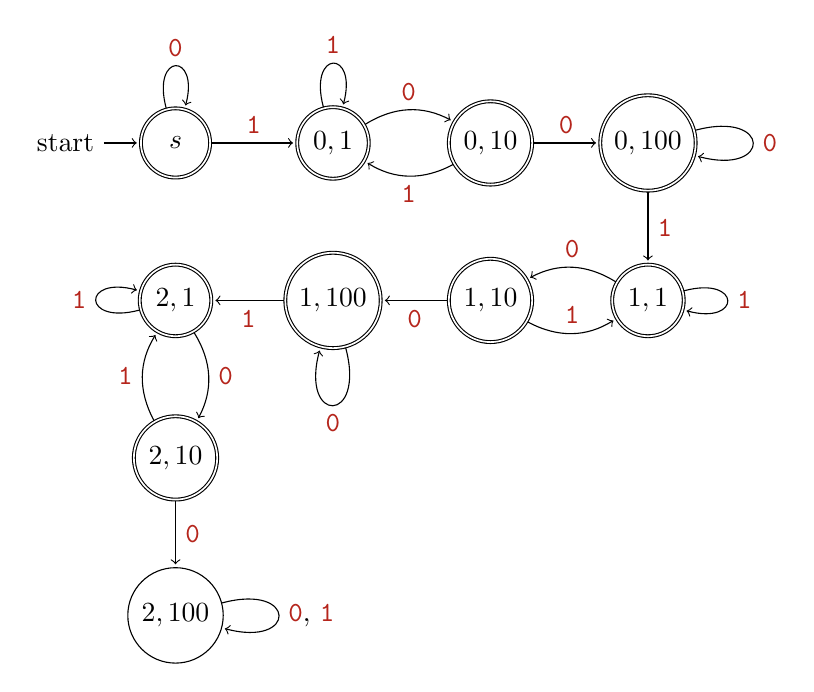
\begin{tikzpicture}[shorten >=1pt,node distance=2cm,on grid,auto] 
   					\node[state,initial,accepting] (s)   {$s$}; 
   					\node[state,accepting] (0_1) [right=of s] {$0,1$}; 
   					\node[state,accepting] (0_10) [right=of 0_1] {$0, 10$}; 
   					\node[state,accepting](0_100) [right=of 0_10] {$0,100$};
   					\node[state,accepting](1_1) [below=of 0_100] {$1,1$};
   					\node[state,accepting](1_10) [left=of 1_1] {$1,10$};
   					\node[state,accepting](1_100) [left=of 1_10] {$1,100$};
   					\node[state,accepting](2_1) [left=of 1_100] {$2,1$};
   					\node[state,accepting](2_10) [below=of 2_1] {$2,10$};
   					\node[state](2_100) [below=of 2_10] {$2,100$};
    				\path[->] 
    				(s)     edge [loop above] node {\Sym0} ()
    					    edge              node {\Sym1} (0_1)
    				(0_1)   edge [loop above] node {\Sym1} ()
    					    edge [bend left]  node {\Sym0} (0_10)
    				(0_10)  edge              node {\Sym0} (0_100) 
          		  		    edge [bend left]  node {\Sym1} (0_1)
          		  	(0_100) edge [loop right] node {\Sym0} ()
          		  			edge				  node {\Sym1} (1_1)
          		  	(1_1)	edge [loop right] node {\Sym1} ()
          		  			edge [bend right, swap] node {\Sym0} (1_10)
          		  	(1_10)  edge [bend right] node {\Sym1} (1_1)
          		  			edge 			  node {\Sym0} (1_100)
          		  	(1_100) edge [loop below] node {\Sym0} ()
          		  			edge 			  node {\Sym1} (2_1)
          		  	(2_1)	edge [loop left]  node {\Sym1} ()
          		  			edge [bend left]  node {\Sym0} (2_10)
          		  	(2_10)	edge [bend left]  node {\Sym1} (2_1)
          		  			edge 			  node {\Sym0} (2_100)
          		  	(2_100) edge [loop right] node {\Sym0, \Sym1} ();
				\end{tikzpicture}
				\caption{DFA that accepts $L$}
        	\end{center}
    	\end{figure}
    	\item $(0^*(\varepsilon + 1)(\varepsilon + 0))^*(100)(0^*(\varepsilon + 1)(\varepsilon + 0))^*(100)(0^*(\varepsilon + 1)(\varepsilon + 0))^*$
    	
    	\textbf{Reason:} Other than two \Sym{100}s, the other parts, if have \Sym{1}, should have no more than $2$ consecutive \Sym{0}s.
	\end{enumerate}
		
\end{solution}

% ---------------------------------------------------------

\HomeworkHeader{1}{3}

\begin{quote}
Let $L_1, L_2,$ and $L_3$ be regular languages over $\Sigma$
  accepted by DFAs $M_1 = (Q_1, \Sigma, \delta_1, s_1, A_1)$,
  $M_2 = (Q_2, \Sigma, \delta_2, s_1, A_2)$, and $M_3 = (Q_3,
  \Sigma, \delta_3, s_3, A_3)$, respectively.

\begin{enumerate}
\item Describe a DFA $M = (Q, \Sigma, \delta, s, A)$ in terms of $M_1,
  M_2,$ and $M_3$ that accepts $L = \{w \mid w$ is in exactly two of
  $\{L_1, L_2, L_3\}\}.$ Formally specify the components $Q, \delta,
  s,$ and $A$ for $M$ in terms of the components of $M_1, M_2,$ and
  $M_3$.
\item Prove by induction that your construction is correct.
\end{enumerate}
\end{quote}
\hrule


\begin{solution}

	\begin{enumerate}
		\item For $M = (Q, \Sigma, \delta, s, A)$ that accepts exactly two of $\{L_1, L_2, L_3\}$,
			
			We require that:
				\begin{itemize}
					\item $Q = Q_1 \times Q_2 \times Q_3$
					\item $\Sigma$ to be the same as $M_1, M_2, M_3$
					\item $\delta: Q \times \Sigma \rightarrow Q$, that $\delta((q_1, q_2, q_3), a) = (\delta_1(q_1, a)), \delta_2(q_2, a), \delta_3(q_3, a)), a \in \Sigma, q_1 \in Q_1, q_2 \in Q_2, q_3 \in Q_3$
					\item $s = (s_1, s_2, s_3)$
					\item $A = (A_1 \times A_2 \times (Q_3 - A_3)) \cup  (A_1 \times (Q_2 - A_2) \times A_3) \cup ((Q_1 - A_1) \times A_2 \times A_3)$
				\end{itemize}
		\item \textbf{Proof:}
			Apply induction on the length of $w$.
			
			Base case: When $|w| = 0$, namely, $w = \varepsilon$, $\delta(s, w) = \delta(s, \varepsilon) = (\delta_1(s_1, \varepsilon), \delta_2(s_2, \varepsilon), \delta_3(s_3, \varepsilon)) = (s_1, s_2, s_3) = s$. 
			
			If $w \in L$, without losing generality we can assume $w \in L_1, L_2$ only, so $\delta_1(s_1, w) = s_1 \in A_1, \delta_2(s_2, w) = s_2 \in A_2, \delta_3(s_3, w) = s_3 \notin A_3$. Thus, $s \in A$, which means $M$ accepts $w$. 
			
			If $M$ accepts $w$, then $s = (s_1, s_2, s_3) \in A$, which means that $s_1 \in A_1, s_2 \in A_2, s_3 \notin A_3$ or $s_1 \in A_1, s_2 \notin A_2, s_3 \in A_3$ or $s_1 \notin A_1, s_2 \in A_2, s_3 \in A_3$. Then exactly $2$ of $M_1, M_2, M_3$ accepts $w$, so $w$ in exactly $2$ of $L_1, L_2, L_3$. Hence, $w \in L$.
			
			Suppose for all $|w| \leq k$, if $w \in L$, then $M$ accepts $w$. And if $M$ accepts $w$, then $w \in L$.
			
			Then when $|w| = k + 1$, let $w = w_0 \Cdot a, a\in \Sigma$, $\delta(s, w) = \delta(\delta(s, a), w_0)$. By induction hypothesis, we know that $\delta(s, a)$ corrected judged if $a$ should be accepted. And let $\delta(s, a) = q$, $\delta(q, w_0)$, since $|w_0| = k$, again, by induction hypothesis, we know that $\delta(q, w_0)$ corrected judged if $w_0$ should be accepted by $M$.
			
			If $M$ accepts $w$, then $\delta(s, w) \in A \Rightarrow (\delta_1(s_1, w), \delta_2(s_2, w), \delta_3(s_3, w)) \in A$. That means that $\delta_1(s_1, w) \in A_1, \delta_2(s_2, w) \in A_2, \delta_3(s_3, w) \notin A_3$ or $\delta_1(s_1, w) \in A_1, \delta_2(s_2, w) \notin A_2, \delta_3(s_3, w) \in A_3$ or $\delta_1(s_1, w) \notin A_1, \delta_2(s_2, w) \in A_2, \delta_3(s_3, w) \in A_3$, so exactly $2$ of $M_1, M_2 , M_3$ accepts $w$, so $w$ in exactly $2$ of $L_1, L_2, L_3$. Hence $w \in L$.
				
			In conclusion, the automata $M$ described above is correct.
	\end{enumerate}
\end{solution}

\end{document}
